%\chapter[Probabilistic neural models and their plausibility]{Neural implementations of uncertainty and inference and their consistency with the hippocampal complex}

\chapter{Additional evidence for sampling-based Bayesian localization}
\label{apx:pfev}

In Chapter 7, we have addressed the observation that there is a subset of neurons in the hippocampus with firing fields which seem to contradict the uncertainty predictions of a Bayesian model. The reasonably god fit to place fields sizes reported in Chapter 4, although imperfect, suggest that some place cells do approximate Bayesian posteriors. However, it is very likely that only a subset does so, and that part of the hippocampus performs different computations altogether.

To show that our sampling-based Bayesian localization model can function even under conditions where a proportion of the samples is corrupted by non-Bayesian processes, we have compared the distribution of uncertainties predicted by the sampling-based model to the distribution of place field sizes.

We have used the implemented sampling-based cognitive model (described in Chapter 6) to replicate the experiment (Burke et al., 2011). In the experiment, rats were running in circles on a circular track with 106cm diameter, which contained 2 food trays to motivate the rats, and no objects in one condition and 8 pseudorandomly distributed, different objects in another condition. The model performed random trajectories in an environment of the same proportions, with the same landmarks. 

Figure \ref{distr} shows the resulting distribution of uncertainties along the track, measured as the standard deviation of all posterior samples (location hypotheses) in the model. These uncertainties are compared to the distribution of place field sizes along the track. Note the matching ratio of the most frequent place field sizes and uncertainties at $21cm$ (objects) and $38cm$ (no objects) respectively, and the roughly matching ratio between all normalized frequencies of occurrence between objects and no objects conditions.

\begin{figure}[!ht]
	\begin{center}
		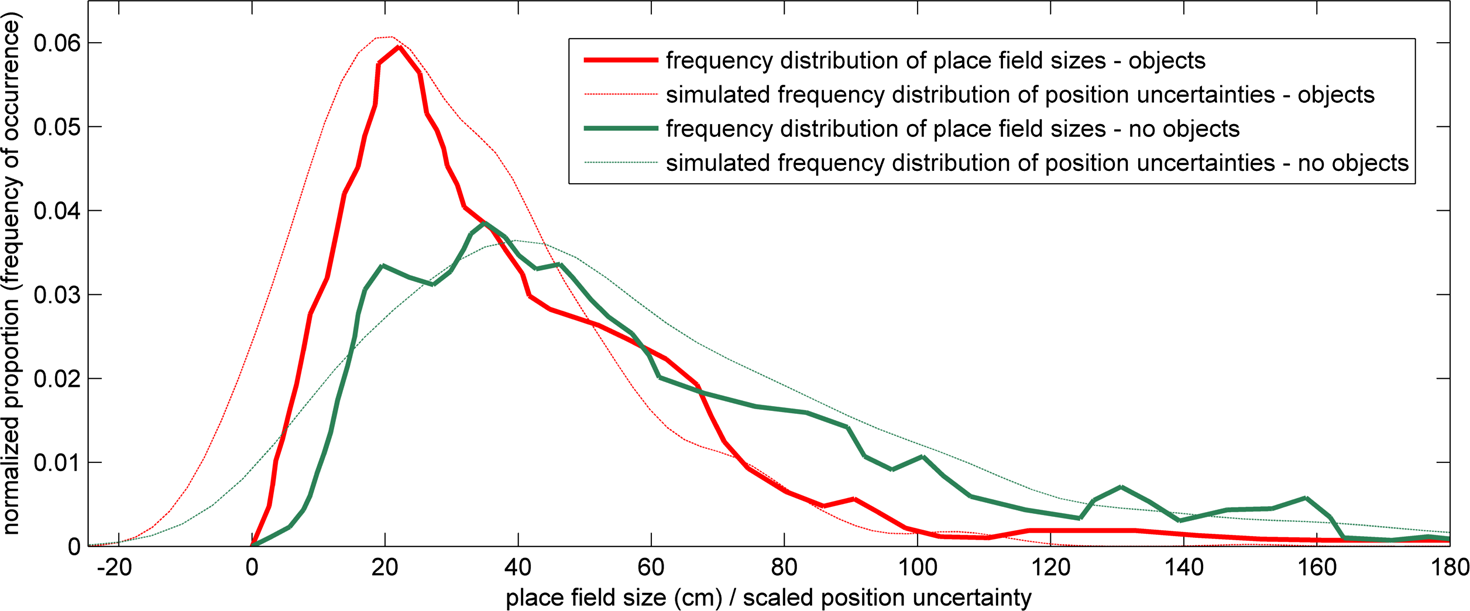
\includegraphics[width=\textwidth]{img/burkefreqdist}
	\end{center}
	\caption{
		{\bf Occurrence frequencies of different place field sizes} in all measured neurons in the no
		objects (blue) and 8 objects (red) conditions, compared to the frequencies of position uncertainties in
		the simulation. Data from (Burke et al., 2011). 
	}
	\label{distr}
\end{figure}



%An appendix is just like any other chapter, except that it comes after
%the appendix command in the master file.
%
%One use of an appendix is to include an example of input to the system
%and the corresponding output.
%
%One way to do this is to include, unformatted, an existing input file. 
%You can do this using \verb=\verbatiminput=. In this appendix we
%include a copy of the C file \textsf{hello.c} and its output file
%\textsf{hello.out}. If you use this facility you should make sure that
%the file which you input does not contain \texttt{TAB} characters,
%since \LaTeX\ treats each \texttt{TAB} as a single space; you can use
%the Unix command \texttt{expand} (see manual page) to expand tabs into
%the appropriate number of spaces. 
%
%\section{Example input and output}
%\label{sec:inp-eg}
%\subsection{Input}
%\label{sec:input}
%(Actually, this isn't input, it's the source code, but it will do as
%an example)
%
%\verbatiminput{hello.c}
%
%\subsection{Output}
%\label{sec:output}
%
%\verbatiminput{hello.out}
%\subsection{Another way to include code}
%You can also use the capabilities of the \texttt{listings} package to
%include sections of code, it does some keyword highlighting.
%
%\lstinputlisting[language=C]{hello.c}

%\bibliography{refs}